\chapter{Further Justification of New Termination Conditions in Section~\ref{Subsec:PLGD_term_crit-new_term_crit}}      		\label{Sec:Appx-further_reasons_for_new_term_crit}



Section \ref{Subsec:PLGD_term_crit-new_term_crit} demonstrated that the primal difference (\ref{Eqn:term_crit-candidate_residuals}e) and dual variable difference (\ref{Eqn:term_crit-candidate_residuals}i) effectively identify the point at which the GDD algorithm (Algorithm \ref{Alg:PGD}) stagnates for PLGD models with Gaussian noise (\ref{Eqn:PhaseLift-GD_Gaussian_noise}).  
This appendix demonstrates that all of the remaining residuals from  (\ref{Eqn:term_crit-candidate_residuals}) are either unreliable or effectively a duplicate of another computationally cheaper residual.  

One residual that may be eliminated is the primal relative error (\ref{Eqn:term_crit-candidate_residuals}d).  The original termination conditions for the GDD algorithm include the feasibility requirement (\ref{Eqn:saga_conv_crit_primal}) 
\begin{equation*}
|| \caA(xx^*) - b ||_2 \leq \epsilon + \textnormal{tol}_\textnormal{feas} (1 + ||b||_2),
\end{equation*}
which is equivalent to the primal relative error (\ref{Eqn:term_crit-candidate_residuals}d) using the relation $\epsilon_\rel = \epsilon / ||b||_2$
\begin{equation}
	\label{Eqn:GD_new_termination_conds-primal_feas}
\frac{||\caA(xx^*) - b||_2}{||b||_2}  \leq \epsilon_\rel + \textnormal{tol}_\textnormal{feas} \left(\frac{1 + ||b||_2}{||b||_2}\right).
\end{equation}
As indicated in Table \ref{Tab:term_crit-pr_feas_faster_for_big_L_noise}, the GDD algorithm typically requires only a few iterations before a primal feasible signal $x$ is found.  Yet in certain cases the GDD algorithm may never identify a feasible signal.  Figure \ref{Fig:term_crit-pr_err_fails} demonstrates plots the primal relative error (\ref{Eqn:term_crit-candidate_residuals}d) for the particular model from Figure \ref{Fig:term_crit-signal_err} which never attained primal feasibility.

\begin{figure}[H]
\centering
\hbox{\hspace{-1.0cm} 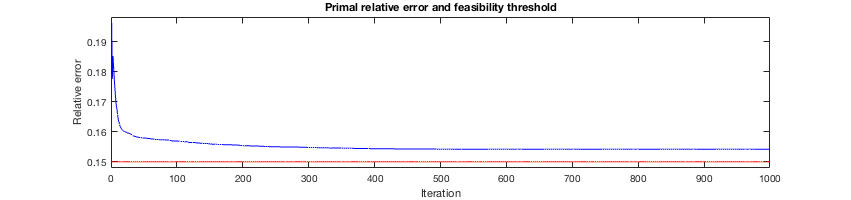
\includegraphics[scale=0.6]{term_crit-pr_err_fails} }
\caption{Primal relative error (\ref{Eqn:term_crit-candidate_residuals}d) (blue) and noise ratio threshold (red) for noise ratio $\epsilon_\rel = 0.15$ and oversampling rate $L = 5$.  Iterate 1,000 remains infeasible with a primal relative error of $0.1541$.}
\label{Fig:term_crit-pr_err_fails}
\end{figure}

% experiments.figure.noisyimage_new_termination_criteria

The experiment in Figure \ref{Fig:term_crit-pr_err_fails} demonstrates a model where both the exact tolerance $\epsilon_\rel = 0.15$ and the relaxed tolerance $ \epsilon_\rel + \textnormal{tol}_\textnormal{feas} \left(\frac{1 + ||b||_2}{||b||_2}\right) =0.1502$ as suggested in (\ref{Eqn:saga_conv_crit_primal}) are unattainable by the GDD algorithm.  Nevertheless, the GDD algorithm makes significant progress in recovering an approximate signal.  Notably, the wflow algorithm applied to the same model recovers a signal with a primal relative error (\ref{Eqn:term_crit-candidate_residuals}d) of $0.3165$.  Thus we ignore the primal feasibility condition (\ref{Eqn:saga_conv_crit_primal}).


We may also disregard the duality gap (\ref{Eqn:term_crit-candidate_residuals}f) as a termination condition.  The experiments in Table \ref{Tab:average_rank_soln_matrix_with_gaussian_dual_variable} demonstrate that the duality gap tends to stagnate at different values for differing noise level and oversampling rate.  Table \ref{Tab:term_crit-duality_gap_stagnates} indicates the final duality gap value for each experiment from Figure \ref{Fig:term_crit-signal_err}, further demonstrating this residual is not a reliable indicator of stagnation.

\begin{table}[H]
\centering
\begin{tabular}{ |c|c|c| }
\hline
&	$L = 5$
	&	$L = 10$	\\
 \hline
$\epsilon_\rel = 0.05$
&     8.24 &   8.10 		\\
 \hline
$\epsilon_\rel = 0.15$
&  39.23 &  29.41 	\\
 \hline
$\epsilon_\rel = 0.30$
&  38.93 &  59.73	\\
 \hline
\end{tabular}
\vspace{0.5cm}
	\caption{Final values of duality gap (\ref{Eqn:term_crit-candidate_residuals}f) after 1,000 iterations of the GDD algorithm (Algorithm \ref{Alg:PGD}) with indicated noise ratios and oversampling rates.}
	\label{Tab:term_crit-duality_gap_stagnates}
\end{table}
% experiments.figure.noisyimage_new_termination_criteria

The duality gap (\ref{Eqn:term_crit-candidate_residuals}f) is not reliable because this measurement is dependent on the accuracy of both the dual objective value $\lambda_1$ and the approximate signal norm $||xx^*||_1$ as compared to their respective optimal values.  As established in Section \ref{Subsec:PLGD_term_crit-stagnation}, the GDD algorithm cannot achieve optimality for most noisy phase retrieval models.  Thus the complementarity condition $||xx^*||_1 \cdot \lambda_1 = 1$ (Corollary \ref{Cor:PLGD-optimality}, d) cannot be achieved.  As a result, the duality gap (\ref{Eqn:term_crit-candidate_residuals}f) stagnates unpredictably for varying oversampling rates and noise levels and is not used as a termination condition for the GDD algorithm.



Next we demonstrate that the duality gap difference (\ref{Eqn:term_crit-candidate_residuals}g) is a redundant measurement.  Denote the primal objective value as $p = ||xx^*||_1$ and its update with a hat.  As the GDD algorithm stagnates, $\hat{p} / p$ approaches $1$. Additionally, note that typical optimal signals have fairly large norms (i.e., $||\mathbf{x}\mathbf{x}^*||_F = \caO(10^3)$ or larger).  If we assume $\hat{p}/p \approx 1$ and $\lambda_1 -  1/p \approx \lambda_1$ for later iterates then we have
\begin{equation}
\begin{split}
\frac{| \gamma - \hat{\gamma}|}{\gamma}	&	=	\frac{| (p \lambda_1 - 1) - (\hat{p}\hat{\lambda}_1 - 1) |}{p \lambda_1 - 1}
		\\
	&	= \frac{\left| \lambda_1 - \frac{\hat{p}}{p}\hat{\lambda}_1 \right|}{ \lambda_1 - \frac{1}{p} }
		\\
	&	\approx \frac{| \lambda_1 - \hat{\lambda}_1|}{\lambda_1}.
\end{split}
\end{equation}

Thus the duality gap difference (\ref{Eqn:term_crit-candidate_residuals}g) behaves similarly to the dual objective difference (\ref{Eqn:term_crit-candidate_residuals}h) and may be disregarded.  

Finally, the dual matrix difference (\ref{Eqn:term_crit-candidate_residuals}j) is also a redundant measurement which may be disregarded.  Note that the norm difference of dual matrices is bounded above by the dual variable difference (\ref{Eqn:term_crit-candidate_residuals}i), since
\[
||A - \hat{A}|| = ||\caA^*(y - \hat{y})|| \leq ||\caA^*|| \ ||y - \hat{y}||_2,
\]
where we have the induced norm of $\caA^*$
\[
||\caA^*|| = \sup_{\substack{||w||_2=1}}||\caA^*w||.
\]
And computationally, the dual variable difference (\ref{Eqn:term_crit-candidate_residuals}i) is computed with a vector norm, where as the dual matrix difference (\ref{Eqn:term_crit-candidate_residuals}j) requires an additional eigenvalue computation (in this case the largest magnitude eigenvalue).  Thus the dual matrix difference (\ref{Eqn:term_crit-candidate_residuals}j) can be ignored due to its excessive computational cost and close relationship to the dual variable difference (\ref{Eqn:term_crit-candidate_residuals}i).



Finally, we may also eliminate the dual objective difference (\ref{Eqn:term_crit-candidate_residuals}h) as a candidate residual for termination.  Figure \ref{Fig:term_crit-dual_obj} depicts the behavior of this residual for the models in Figure \ref{Fig:term_crit-signal_err}.  As with Figure \ref{Fig:term_crit-pr_and_dual}, the vertical axis indicates specific tolerances and the horizontal axis indicates the first iterate at which the GDD algorithm would satisfy this tolerance.


\begin{figure}[H]
\centering
\hbox{\hspace{-1.5cm} 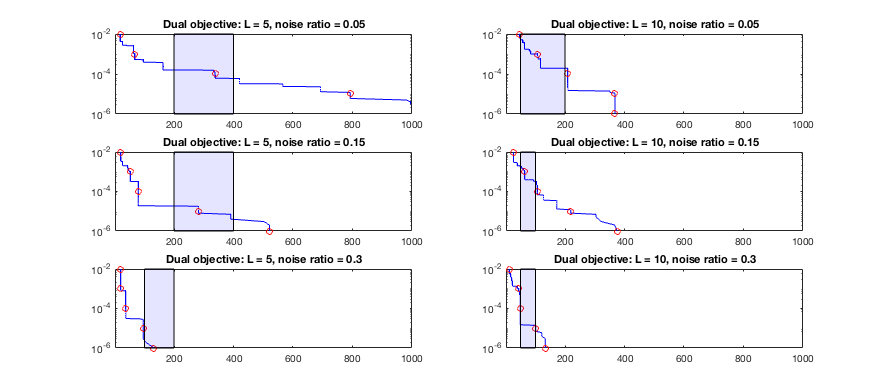
\includegraphics[scale=0.6]{term_crit-dual_obj} }\vspace{-0.4cm}
\caption{Plots of dual objective difference values (\ref{Eqn:term_crit-candidate_residuals}h) against the iterate at which the GDD algorithm (Algorithm \ref{Alg:PGD}) first satisfies this tolerance for the models discussed in Figure \ref{Fig:term_crit-signal_err}.  Red circles are placed at tolerances $10^{-n}$.  The blue rectangles indicate the proposed intervals of termination from Table \ref{Tab:term_crit-desired_termination_windows}.}
\label{Fig:term_crit-dual_obj}
\end{figure}
% experiments.figure.noisyimage_new_termination_criteria


Figure \ref{Fig:term_crit-dual_obj} demonstrates that the dual objective difference (\ref{Eqn:term_crit-candidate_residuals}h) behaves erratically, decreasing too slowly for low-noise models and too quickly for high-noise models.  To simplify our discussion, label the dual objective tolerance as $\tol_\text{DO}$.  If we set $\tol_\text{DO} = 10^{-5}$, then the GDD algorithm will terminate far too late for the top-left model in Figure \ref{Fig:term_crit-dual_obj}.  However, if we set $\tol_\text{DO} = 10^{-4}$ then the GDD algorithm may terminate far too early for the middle-left and bottom-left models.  Likewise, the models at right in Figure \ref{Fig:term_crit-dual_obj} do not have a consistent tolerance value $\tol_\text{DO}$ which reliably selects for termination within the desired intervals.  Thus the tolerance $\tol_\text{DO}$ is not a reliable indicator of stagnation of the GDD algorithm. 



